% !TeX spellcheck = en_US
\documentclass[11pt, fleqn, titlepage]{article}
%\usepackage{siunitx}
\usepackage{texfiles/SpeedyGonzales}
\usepackage{texfiles/MediocreMike}
\newcommand{\so}[2]{{#1}\mathrm{e}{#2}}
% \geometry{top=1cm}
\usepackage{hyperref}
\usepackage{amsmath}
\usepackage{ragged2e}
\usepackage{booktabs}
\usepackage{lipsum}
\usepackage{csquotes}
\usepackage{longtable}
\usepackage{arydshln}
\usepackage{subcaption}
\usepackage{listings}
\usepackage{pxfonts}
\lstset{
	basicstyle=\ttfamily,
	keywordstyle=\bfseries,
	showstringspaces=false,
	morekeywords={def, for, return, if, else},
	xleftmargin=-3.0cm
}
\hypersetup{
	colorlinks=true,
	linkcolor=blue,
	filecolor=magenta,      
	urlcolor=cyan,
}
\usepackage{nccmath}
\usepackage{multicol}
%\usepackage{subfig}
\usepackage{graphicx}
%\usepackage{algorithmic}
%\usepackage{program}
\title{Fairness in Classification}
\author{Anders Henriksen \\ Oskar Eiler Wiese Christensen  \\ \texttt{\{s183917, s183904\}@student.dtu.dk}}
\date{\today}

\pagestyle{plain}
\fancyhf{}
\rfoot{Page \thepage{} of \pageref{LastPage}}

\graphicspath{{Billeder/}}

\begin{document}
	
	\maketitle
	\begin{abstract}
		\textbf{TODO: Skal indeholde motivation, problem, fremgangsmåde, resultater og konklusion.} \\ \lipsum[1-2]
	\end{abstract}
	\tableofcontents \newpage
	%\thispagestyle{fancy}
	%\tableofcontents	
	
	\section{Introduction} \label{indledning}
	%\textbf{TODO: \\ Hvad er formålet med projektet? \\ Hvad er problemformuleringen \\ Hvad er state-of-the-art? \\ Hvilken fremgangsmåde bruges til at løse problemet? \\ Hvem har brug for resultaterne?}
	
	\subsection{Motivation}
	%TODO 
	%Der skal skrives mere aktuelt om situtationen i USA 
	Artifical intelligence (AI) and machine learning (ML) methods are playing a bigger and bigger role in modern society. As the accuracies of AI and ML models increase, their applications become wider, allowing for these  models to be implemented either as ground truth or as a pointer in applications like autonomous vehicles, medical imaging, the American judicial system ect. These models are, for the general public, often seen as an objective decision maker. As such, it becomes of essence to avoid discrimination, since model discrimination could lead to reinforced societal discrimination. Bias seems to originate from the dataset, meaning that a saving grace would be to either implement bias correction on the dataset to remove the bias from the source of the problem or to remove bias from the model, thereby removing the risk of discrimination when using the model for classification tasks. This report aims to understand bias and how it affects datasets as well as classification models. Furthermore, bias correction methods will be put to use in order to explore the possibilites of keeping discrimination away from important fields. More specifically, the questions to be answered throughout the report are whether there is a bias in the COMPAS recidivism dataset and which kind of bias there is, as well as what this bias means in the dataset. Meanwhile, it is also analyzed how bias affects a binary classification feed-forward neural network algorithm, how bias in an algorithm is detected and how to quantify the bias. Lastly, bias correction methods will be implemented and tested and an ethical discussion will be carried out to understand the applications of bias correction algorithms and AI models on society as well as how society can learn to trust these models. \\
	
	\noindent In this report, the rest of section \ref{indledning} will focus on related work within the field of bias correction and the contributions from this report. Afterwards, section \ref{data} will present the necessary details of the COMPAS dataset including visualizations of possibly discriminatory variables like "race" and "sex", explanations of the variables of the dataset and how the data was collected and put together. Section \ref{methods} on methods sets up the necessary background knowledge for the topics of FFNNs, permutation tests, bias identification and bias correction methods. The section will also contain a description of how to reproduce the results. Results will be illustrated in section \ref{results} through figures and tables, which will then be discussed and put into a greater perspective in section \ref{discussion}. The discussion also contains the ethical discussion of bias and bias correction as a whole. The whole report will be summed up in section \ref{conclusion}. Some lesser relevant figures and points as well as pseudo code for some of the used functions have been left out of the report, but can be found in section \ref{appendix} and the relevant sources are found in section \ref{bibliography}.
	
	\subsection{Equal Opportunity and Equalized Odds}\label{bias_def}
	
	The two main fairness definitions used in this project are proposed by Hardt et. al \cite{equal_of_oppor}.\newline \textbf{Definition 1.1}(Equalized Odds)\textbf{:} A given predictor $ \hat Y $ satisfies equalized odds with respect to the protected attribute A and outcome $ Y $, if $ \hat Y $ and A are independent conditional on Y. If the target is binary, then equalized odds can be expressed mathematically as
	\begin{equation*}\label{key}
	\operatorname{Pr}\{\widehat{Y}=1 | A=0, Y=y\}=\operatorname{Pr}\{\hat{Y}=1 | A=1, Y=y\}, \quad y \in\{0,1\}.
	\end{equation*}
	What equalized odds states is that if $ \hat Y $ has to be a fair predictor, then if $ y = 1 $ the predictor has to have equal true positive rates for both classes of A, i.e. $ A = 0 $  and $ A = 1 $. However, if $ y = 0 $ then the predictor $ \hat Y $ has to have equal false positive rates. Equalized odds ensures equal accuracy and bias in all classes, and punishes models that perform well only on the majority.
	\\\\
	\textbf{Definition 1.2}(Equal Opportunity)\textbf{:} A binary predictor $ \hat Y $ satisfies equal opportunity with respect to A if 
	\begin{equation*}
		\operatorname{Pr}\{\hat{Y}=1 | A=0, Y=1\}=\operatorname{Pr}\{\hat{Y}=1 | A=1, Y=1\}.
	\end{equation*}
	Equal opportunity ensures that the probability of predicting $ \hat Y = 1 $ is equal across the classes given the fact that $ Y = 1 $. Equal opportunity is a weaker notion of non-discrimination than Equalized Odds, but still allows for better utility than implementing no bias correction method at all.
	
	
	\subsection{Related Work}
	There are currently two main ways to ensure fairness in classification. One of the ways is by implementing steps during the training process of the classifier in order to ensure fairness definitions. The second method, which is the one which will be implemented in this project, involves post-processing steps. Post-processing methods are often desired because the method can be used on models that have been trained and are commercialized. With the vast increase of Machine Learning models on the market, society calls for ways to ensure that these models do not discriminate any minority or anyone for that matter. Many different suggestions of how to implement bias correction algorithms within the field of fair AI have been proposed in the last years. However, this is still a young field of science with many improvements to come.\\\\
	\noindent
	An approach proposed by Zafar et al. \cite{Zafar}, suggests that a way to achieve fair classifiers is by using linear constraints on the covariance between predicted labels and the value of features. This is a method that is implemented during the training process, which means that trained algorithms would have to be retrained. "Satisfying Real-world Goals with Dataset Constraints" uses the same strategy to remove bias inheritance from the dataset, which is to use linear constraints. The study proposes constraints in the training data, and by using the ramp penalty to quantify cost accurately, they succeed in developing an efficient algorithm to optimize the resulting non-convex constrained optimization problem. This state-of-the-art algorithm can be implemented in situations where one may require a classifier to make predictions with a certain rate of positive predictions in order to maintain fairness for a population. Equality of opportunity is one of such definitions which require the true positive rates of protected attributes to be equal. \cite{g_goh} \\
	
	\noindent The main method that will be demonstrated in this project is proposed by Hardt et al. \cite{equal_of_oppor}. The suggested method can achieve a non-discriminatory classifier by a post-processing step. The idea is to learn thresholds in order to deal with sensitive features or groups in the data in a discriminant classifier. The method requires that the classifier has information about the data at decision-time, which is the case in the experiment conducted in this project. The study proposes, that with the learned thresholds, they can ensure fairness definitions (see section \ref{bias_def}) by using different thresholds for certain protected groups. However, another article, namely "Learning Non-Discriminatory Predictors", argue that by only using the post-hoc correction (post-training methods), the algorithm will still be unfair. \cite{b_woodworth} They show that for several loss functions such as the 0-1 or hinge loss, the method proposed by Hardt et al. \cite{equal_of_oppor} can fail. In the paper, a notion is defined to obtain an approximation of a non-discrimination algorithm. However, this notion is explored during the paper, and it turns out that creating a non-discrimination algorithm is computationally hard. Therefore, a relaxation definition of equalized odds is presented, which is based on a second-moment condition instead of full conditional independence. Throughout the paper, it is shown that under this condition it is possible to learn a nearly optimal non-discriminatory linear predictor with respect to a convex loss without it being too computational to train. \cite{b_woodworth}\\\\
	The scope of this project is to implement the post-hoc correction method presented by Hard et al. \cite{equal_of_oppor} on a binary classifier trained on the COMPAS dataset. The goal is to obtain a non-discriminatory classifier which still retains a respected accuracy. The motivation behind implementing the work of Moritz Hardt is due to his great success within the field of fairness in Machine Learning. Hardt has more than 7000 citations, is currently writing a book about fairness in ML and has several scientific studies, including Equality of Opportunity in Supervised Learning. Moreover, the fairness definition of Equalized Odds, Equality of Opportunity and Demographic Parity are currently well accepted fairness definitions. Thus, the benefits and trade offs of using Hard et al.'s definitions will be discussed and examined thoroughly.
	
	\subsection{Contributions}
	This report aims to give an approachable account of the effects of bias as well as the most promising methods of removing bias and avoiding discrimination from learned supervised learning models in datasets. As such, the reader can expect to get the following from this report.
	
	\begin{itemize}
		\item Illustrations which show an overview of the possible bias present in the modified COMPAS recidivism dataset. The effect of how this possibly biased data affects a classifier will be examined in this report. 
		\item A comprehensive table of all variables present in the modified COMPAS recidivism dataset will be provided. This table includes the name of the variable, a short description of the purpose of the variable as well as the type of variable in order to remove ambiguity for the definitions of the variables which was previously present.
		\item Two bias correction methods, equalized odds and equal opportunity, will be presented, both through text and mathematical definition, and implemented in order to show the effect of the bias corrections on a binary neural network classifier.
		\item To put the other contributions into a real-world context, an ethical discussion of the quantified bias and discrimination models will be carried out.
		\item Pseudo code for the implementation of equal opportunity and equalized odds as well as a section on reproducibility will be provided in the interest of making the results of this paper both as replicable and as reliable as possible. The section on reproducibility supplies the reader with the used seeds, packages, versions of these packages and a thorough explanation of the code used to make the project come to life.
	\end{itemize}
	The general goal of the contributions given above is to avoid models that discriminate with respect to some protected attribute. In this report, race plays the biggest role as a protected attribute, but the findings of the discriminating models and bias correction can equally be transferred to other variables that are suspected to be discriminated against. This could be variables such as nationality, sex, income, sexual orientation etc.
	
	\section{Data} \label{data}
%	\textbf{TODO: \\ Data kan kort introduceres i indledningen \\ Lav etisk diskussion om opbevaring af data samt privacy issues}
	
	\noindent To analyse the efficacy of using bias correction to remove discrimination among races in the American justice system, the modified COMPAS recidivism dataset from ProPublica has been used. An important note on the further work in this report on the dataset is that the output variable \texttt{score\_text} has been turned into a binary vector. This method was also used by ProPublica during their analysis and therefore, turning the output into a binary vector, was logical. The idea was to recreate the algorithm proposed originally by ProPublica. The binarization was performed by merging the \texttt{Medium} and \texttt{High} risk of recidivism into zeros and the \texttt{Low} risk of recidivism into ones. \\
	A general overview of the dataset and how it came to be as well as the variables used for the classifier is given in section \ref{dataDescription}. The data and variables have not been properly explained to any extent in examined literature, so section \ref{dataExamination} will cover the meaning of all 53 variables of the dataset to remove ambiguity and set a common ground from which to base the future analysis. Lastly, section \ref{dataVisuals} will show important visualizations of features of the dataset to cover which of the variables are most likely to contain biases that will be explored and examined further in later sections.
	
	\subsection{Description of Data} \label{dataDescription}
	The data used in this project stems from an initial analysis of the COMPAS (Correctional Offender Management Profiling for Alternative Sanctions) algorithm by its developers, Northpointe Inc. After this analysis, ProPublica made a subsequent analysis of this data as well as their own queries of the offenders involved and data of the offenders who actually recidivated. This data is stored in the \texttt{compas-scores-two-year.csv} dataset from ProPublica's GitHub page, which can be found here: \url{https://github.com/propublica/compas-analysis/blob/master/compas-scores-two-years.csv}. \\\\
	\noindent The data consists of 53 different variables, 9 of which are used in the binary classification model. Four of the chosen variables are categorical, so these will have to be one-out-of-k encoded in order for the neural network to comprehend them. Meanwhile, the numerical variables, of which there are also four, will be normalized as to avoid the vanishing gradient problem and to avoid having some variables be of more importance to the final prediction. This will be explained more thoroughly in section \ref{Feed-forward neural}. %TODO skriver vi mere thoroughly om det her i metoder?!?\\
	The 10 chosen variables, of which one will be used as the target variable are shown and explained below. To see an exhaustive explanation of all variables from the full dataset, see section \ref{dataExamination}.
	
	
	\begin{table}[H]\label{resultater}
		\centering
		\begin{tabular}{l l l}
			Variable & Description & Type \\ \hline
			age & The age of the offenders & Continuous ratio \\
			priors\_count & The number of previous offences & Discrete interval \\
			juv\_fel\_count & The number of previous juvenile felonies & Discrete interval \\
			juv\_misd\_count & The number of previous juvenile misdemeanor & Discrete interval \\
			c\_charge\_degree & The severity of the offence & Discrete nominal \\
			race & The race of the offender & Discrete nominal \\
			age\_cat & The age category of the offender & Discrete nominal \\
			sex & The sex of the offender & Discrete nominal \\
			score\_text & The COMPAS prediction of chance of recidivism & Discrete interval
		\end{tabular}
		%\caption{text}
	\end{table}
		
		
	\subsection{Explanation of Data Variables} \label{dataExamination}
	Using and researching the extended COMPAS dataset has shown that there is no documentation of the meaning of the variables. This makes interpretation difficult and can make singular variables of the dataset next to impossible to understand. To remove ambiguity about the meaning of the variables, an exhaustive description of every variable and variable type has been produced. This allows for the results of this report to be contained within this interpretation and shines light on the true contents of the dataset. Some variables, mostly those with \textit{c\_}, \textit{r\_} or \textit{vr\_} prefixes,have been grouped together in the table, as these serve the same purpose in the dataset for \textit{custody}, \textit{recidivism} and \textit{violent recidivism} cases respectively. 
	
	\noindent Some variable names have the prefix \textit{v\_}, which has been disregarded as an error. As such, this interpretation of the dataset assumes that these variables are akin to those with the \textit{vr\_} prefix, representing the variables related to violent recidivism. Furthermore, in the case of a few of the variables in the dataset, it has simply not been possible to find a meaningful interpretation, since the entire column is either full of NaN's like in the case of \textit{violent\_recid} or every value of the column one to one with another variable, which is the case between \textit{decile\_score} and \textit{decile\_score\_1} as well as \textit{priors\_count} and \textit{priors\_count\_2}. These variables are kept in the table for completeness but seem to have no discernible purpose in the dataset.
	
	
	\begin{longtable}{l l l} \label{allVars}
		\centering
		Variable & Description & Type \\ \hline
		id & Index of the column & Discrete interval \\
		name & Full name of the offender & Discrete nominal \\
		first & First name of the offender & Discrete nominal \\
		last & Last name of the offender & Discrete nominal \\
		compas\_screening\_date & The date the COMAS score was given & Discrete nominal \\
		sex & The sex of the offender & Discrete nominal \\
		dob & The offender's date of birth & Discrete nominal \\
		age & The offender's age & Continuous ratio \\
		age\_cat & Which age category the offender belongs to & Discrete nominal \\
		race & The offender's race & Discrete nominal \\
		juv\_fel\_count & The number of previous juvenile felonies & Discrete interval \\
		juv\_misd\_count & The number of previous juvenile misdemeanor & Discrete interval \\
		juv\_other\_count & The other types of previous juvenile crimes & Discrete interval \\
		days\_b\_screening\_arrest & ----- & Discrete interval \\ \hdashline
		priors\_count & The number of previous offences & Discrete interval \\
		priors\_count\_2 & & \\ \hdashline
		c\_jail\_in & The date the offender was jailed & Discrete nominal \\
		r\_jail\_in & & \\ \hdashline
		c\_jail\_out & The date the offender was removed from jail & Discrete nominal \\
		r\_jail\_out & & \\ \hdashline
		c\_case\_number & The offense case number & Discrete nominal \\
		r\_case\_number & & \\
		vr\_case\_number & & \\ \hdashline
		c\_offense\_date & The date the offense was performed & Discrete nominal \\
		r\_offense\_date & & \\
		vr\_offense\_date & & \\ \hdashline
		c\_charge\_degree & The severity of the offense & Discrete nominal \\
		r\_charge\_degree & & \\
		vr\_charge\_degree & & \\ \hdashline
		c\_charge\_desc & The offense that was performed & Discrete nominal \\
		r\_charge\_desc & & \\
		vr\_charge\_desc & & \\ \hdashline
		c\_arrest\_date & ----- & Discrete nominal \\
		c\_days\_from\_compas & ------ & Discrete interval \\
		r\_days\_from\_arrest & Recidivism days until arrested for the crime & Discrete interval \\
		violent\_recid & Completely empty data column & NaN \\ \hdashline
		is\_recid & Whether the offender truly recidivated after two years (0/1) & Discrete nominal \\
		is\_violent\_recid & & \\
		two\_year\_recid & & \\ \hdashline
		type\_of\_assessment & What the COMPAS algorithm predicted for the offender & Discrete nominal \\
		v\_type\_of\_assessment & & \\ \hdashline
		decile\_score & Value from 1-10 representing risk of recidivism & Discrete ordinal \\
		decile\_score\_1 & & \\
		v\_decile\_score & & \\ \hdashline
		score\_text & decile score split into three categories & Discrete interval \\
		v\_score\_text & & \\ \hdashline
		screening\_date & When the offender was given the assessment & Discrete nominal \\
		v\_screening\_date & & \\ \hdashline
		in\_custody & When the offender was placed in custody & Discrete nominal \\
		out\_custody & When the offender was removed from custody & Discrete nominal \\
		start & The day the screening started compared to the start of the process & Discrete interval \\
		end & The day the screening ended compared to the start of the process & Discrete interval \\
		event & ------ & Discrete interval
	\end{longtable}
		
	\subsection{Visualization of Data} \label{dataVisuals}
	To better get an understanding of the data, a range of plots are shown below. Figure \ref{fig:predictedrecidrace} aims to show whether there is a difference between the fraction of Caucasians and African-Americans that are predicted by the COMPAS classifier as having low, medium and high risk of recidivism. Figure \ref{fig:predictedrecidsex} has the same purpose, utilizing sex instead of race. Figure \ref{fig:truerecid} \& \ref{fig:proirs} give some insight into the actual amount of crime done by African-Americans and Caucasians and whether the amounts seem to be similar.
	
	\begin{figure}[H]
		\centering
		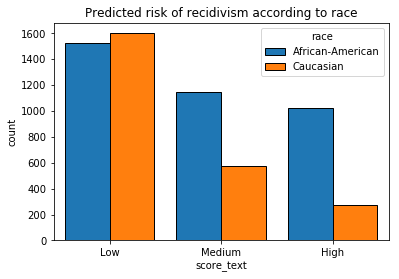
\includegraphics[width=0.5\linewidth]{imgs/predicted_recid_race}	
		\begin{table}[H]
			\centering
			\begin{tabular}{|l|l|l|l|}
				\hline
				& Low   & Medium & High  \\ \hline
				Caucasian        & 0.652 & 0.236  & 0.112 \\ \hline
				African-American & 0.412 & 0.311  & 0.277 \\ \hline
			\end{tabular}
		\end{table}
		\caption{It is clear from this illustration that the number of caucasian and african-american people in the low group are almost equal. Meanwhile the medium and high groups contain a much larger fraction of african-americans. Since, in total, there are more african-americans in the dataset than whites (3696/2454), it would seem based purely on the data that whites are more often classified as low risk of recidivism while african-americans are often classified as medium or high risk.}
		\label{fig:predictedrecidrace}
	\end{figure}

	
	\begin{figure}[H]
		\centering
		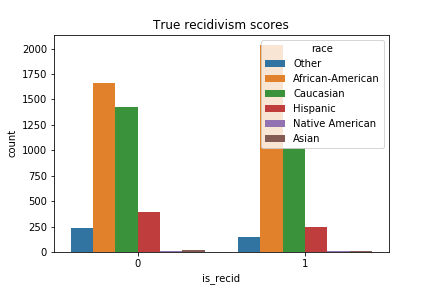
\includegraphics[width=0.5\linewidth]{imgs/true_recid}
		\begin{table}[H]
			\centering
			\begin{tabular}{|l|l|l|}
				\hline
				& 0   & 1  \\ \hline
				Caucasian        & 0.582 & 0.418  \\ \hline
				African-American & 0.449 & 0.551  \\ \hline
			\end{tabular}
		\end{table}
		\caption{This illustration shows the true recidivism values (0 being no recidivism after two years and 1 being recidivism) for all offenders in the dataset seperated by the race of each offender. It is clear that close to an equal amount of white and african-american offenders did not recidivate, while a much larger proportion of african-americans re-offended than whites. This makes it difficult to prove bias in the data based only on the data, as it is not necessarily a bias that african-americans more often re-offend.}
		\label{fig:truerecid}
	\end{figure}
	
	\begin{figure}[H]
		\centering
		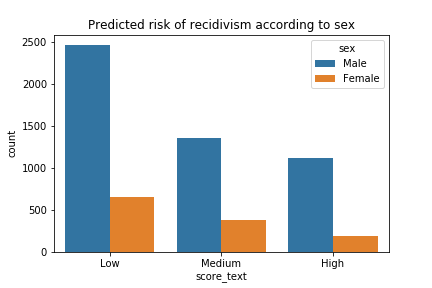
\includegraphics[width=0.5\linewidth]{imgs/predicted_recid_sex}
		\begin{table}[H]
			\centering
			\begin{tabular}{|l|l|l|l|}
				\hline
				& Low   & Medium & High  \\ \hline
				Male      & 0.500 & 0.274  & 0.226 \\ \hline
				Female    & 0.540 & 0.301  & 0.152 \\ \hline
			\end{tabular}
		\end{table}
		\caption{This illustration shows the relationship between sex and the COMPAS prediction of recidivism. The first point to be noted is that there are a lot more men in the dataset than women (5819/1395). Aside from this, it does not seem like there is a difference in the proportions of men or women being classified as belonging to each of the categories.}
		\label{fig:predictedrecidsex}
	\end{figure}
	
	\begin{figure}[H]
		\centering
		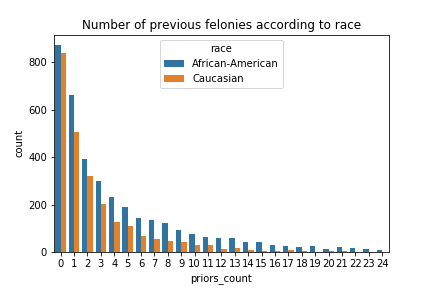
\includegraphics[width=0.5\linewidth]{imgs/proirs}
		\caption{An illustration of the relation between race (african-american or caucasian) and the number of previous felonies prior to the study taking place. This plot gives a clear indication that the number of whites and african-americans who have performed no prior felonies is similar. Otherwise, it is clear that the proportion of african-american to whites becomes larger as the number of previous felonies becomes larger. This seems to indicate that african-americans are more often engaged in criminal activity, which also weakens the indication of a bias from figure \ref{fig:predictedrecidrace}.}
		\label{fig:proirs}
	\end{figure}
	
	
	
	\subsection{Data Origin}
	The COMPAS dataset as well as ProPublica's expanded data and analysis of this data is freely available from their public GitHub repository. As such, the data is not stored safely. This is also true for the variables of the data such as age, full name and number of previous felonies, which give ample opportunity to identify people who have recidivated, leading to compromise of their personal data. This is not a concern though, as the data is collected from Florida, where public records are subject to the broad legislated public right of inspection. According to chapter 119 section 1 of the law of the State of Florida, 
	\begin{displayquote}
		"It is the policy of this state that all state, county, and municipal records are open for personal inspection and copying by any person. Providing access to public records is a duty of each agency." \cite{floridaLaw}
	\end{displayquote}
	
	\noindent As such, since ProPublica submitted a public records request for access to the data for use in research \cite{propublicaAnalysis}, which inherently is a type of inspection, they are within the legal ramifications to use the dataset as they please. Another debate entirely, which will in particular be discussed in section \ref{discussion}, is the more subjective question of the ethicality of open-record laws and public criminal data in their entirety being shared among whomever and what exactly should be allowed to be done with this data.
	
		
	\section{Methods} \label{methods}
%	\textbf{TODO: \\ referér til kode og software \\ brug lang tid på nye %metoder, kort tid på gamle metoder}
	
	\subsection{Binary Classifier}\label{Feed-forward neural}
	%initialization schemes
	\subsubsection{Feed-forward Neural Network}
	Feed-forward neural networks (FFNN) are the simplest kind of neural network. The flow of information in a feed-forward neural network is one-directional, which means that the network has an input layer, and information flow from these nodes through the hidden layers unto the output layer. The main purpose of a FFNN is to approximate a function. In this project $ y = f^*(x) $ maps an input $ \mathbf x $ to a category $ \mathbf y $. The FFNN is thereby a classifier, the goal of which is to determine the recidvism risk of a person given the input variable $ \mathbf x $. $ \mathbf x $ contains both categorical and continuous variables. The categorical variables that are fed to network are the following: \texttt{["c\_charge\_degree", "race", "age\_cat", "sex"]} and the continuous variables are \texttt{["age", "priors\_count", "juv\_fel\_count", "juv\_misd\_count"]}. Most of the other variables contains dates, and would as such make it computationally inefficient to train the network, as one-out-of-k encoding dates takes a lot of rows. The possible values of $ \mathbf y $ are 0 or 1, which corresponds to the classifier classifying a person as either low risk or medium/high risk of recidivism respectively. Hence, this is a binary classifier which constructs a mapping $ \mathbf y = f(\mathbf x \ ; \mathbf w) $. The goal of the FFNN is to learn the weights that most efficiently approximate the function $ f^* $ through supervised learning. The binary classifier in this project has an input layer, five hidden layers and an output layer. \cite{dl}
	
	\begin{figure}[H]
		\centering
		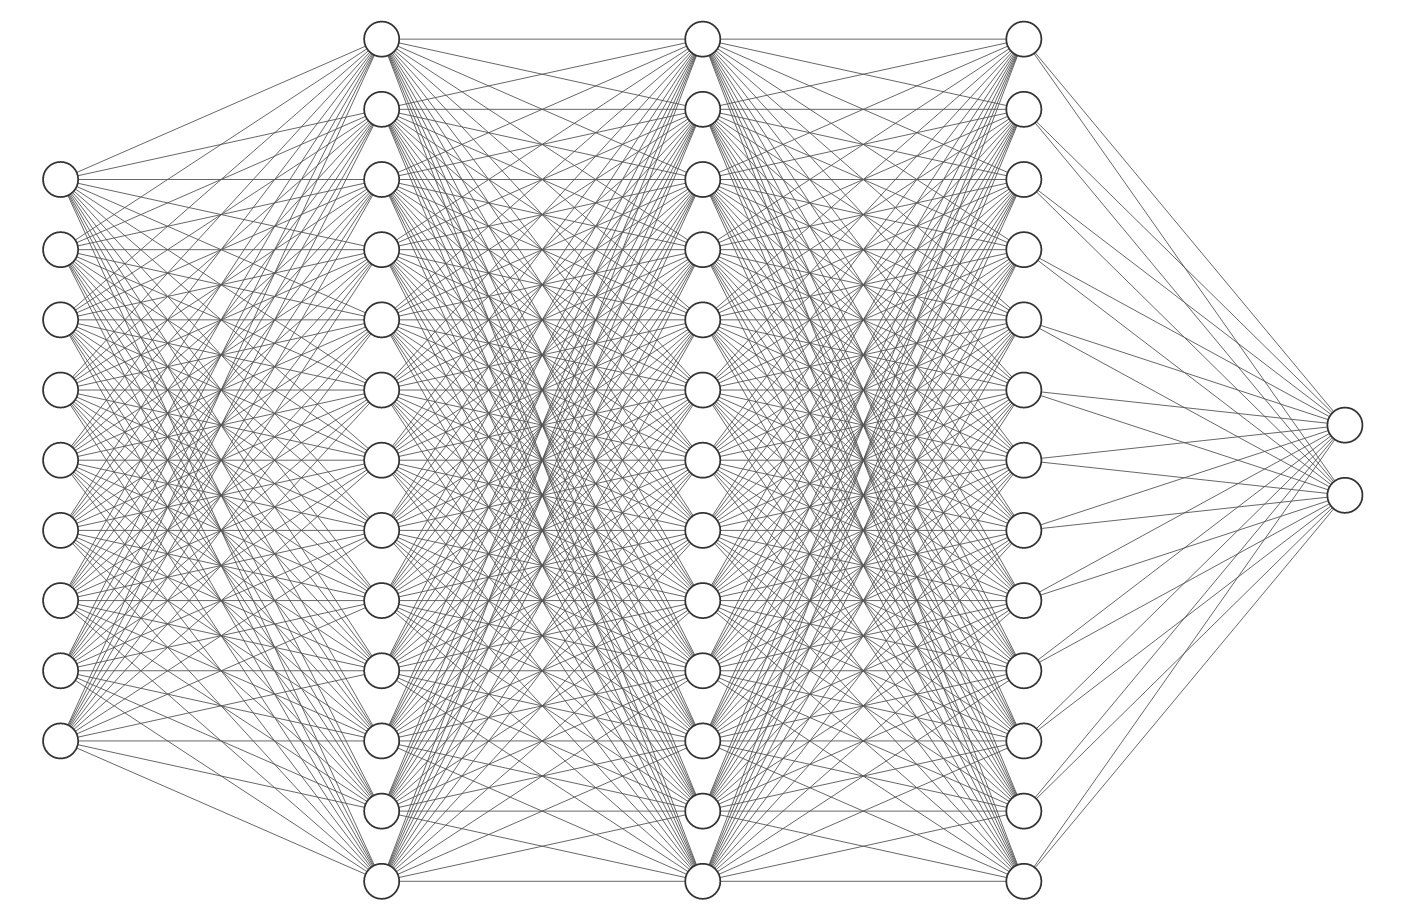
\includegraphics[scale=0.8]{imgs/ffnn}
		\caption{Visualization of the binary classifier model. The input layer has dimension $ \mathbb R ^8$ and the output layer has dimension $ \mathbb R^1 $. The number of nodes in the hidden layers are hyperparameters. The number of nodes used in this project are, layer one through five respectively: $ \mathbb R ^{16} $, $ \mathbb R ^{32} $, $ \mathbb R ^{64} $, $ \mathbb R ^{128} $, $ \mathbb R ^{64} $}
		\label{fig:ffnn}
	\end{figure}
		
	\noindent 
	To obtain the pinnacle of accuracy in a neural network, it needs an excellent architecture as well as the optimal hyperparameters. However, the search for these parameters is usually a costly process of uncertainty, balancing exploration of parameters and the exploitation of previous results. Often, the process of finding the optimal parameters and network architecture comes from expert knowledge, biased heuristics or exhaustive sampling from the parameter space. Since the scope of this project is to demonstrate biased algorithms, the goal is to construct a classifier with an accuracy vastly better than random. The hyperparameters used for the model in this project are based on preliminary runs as well as an exhaustive search through the parameter space. The fully connected layers are trained on the COMPAS dataset with a supervised learning strategy. The hyperparameters used are a drop-out value at $p=0.5$, which is used on each layer. The learning rate, $\alpha$, is initialized as $\alpha = 0.001$. However, the optimization algorithm used for this project is Adaptive Moment Estimation (Adam). Adam is a well known optimizer in the literature and has an adaptive learning rate and step size. The activation function used is rectified linear unit (ReLU), which is defined as $ y = \text{max}(0,x) $. Thus, the function returns x for positive values and zero otherwise. The activation function ensures non-linearity which allows for a more expressive model. Binary Cross-Entropy Loss (BCL) is used as the cost function. The loss in the binary classifier is calculated using the expression below. 
	\begin{equation}\label{key}
	L\left(\boldsymbol{y}_{i}, \hat{\boldsymbol{y}}_{i}\right) = -(\mathbf y \log (\mathbf {\hat y})+(1-\mathbf  y) \log (1-\mathbf {\hat y}))
	\end{equation}
	BCL punishes the algorithm if the predicted value is far from the label. I.e. if the classifier predicts 0.09 and the label is 1, it would result in a very high loss. The ideal model would have a binary cross-entropy loss of zero. \cite {dl} The result is a FFNN with one output node where a threshold can be set, to manipulate how the network will classify an input \textbf{x}. This will be elaborated upon further in section \ref{biascorr}.

	
	\subsection{Permutation test}
	To identify both whether or not the dataset is biased, and if the accuracy of the FFNN is statistically significant, a permutation test was conducted. It is implemented by permuting every variable in the dataset a some number of times and then validating the permuted data with a trained classifier. If the newly acquired accuracy from the permuted data is different from the non-permuted accuracy, this could possibly mean that the classifier is biased. To phrase differently, if the classifier has a tendency to classify Afro-Americans as medium/high risk, a permuted race variable would yield a lower accuracy than the non-permuted data. However, it might just be the reality that all Afro-Americans have a higher chance of recidivism than Caucasians people. Thus, further investigations have to be performed to prove the existence of actual bias in an algorithm. \\\\
	Permutation tests can also be used to validate whether an accuracy from a model is statistically significant. When the model is trained on the COMPAS dataset with supervised learning and a validation accuracy has been obtained, it is important to know if the model performs better than random, which can be evaluated using a permutation test. A null hypothesis $H_{0}$, stating that the observed value comes from the distribution of randomized permutations, is set up and evaluated. To attempt to reject the null hypothesis, each input variable was shuffled randomly and the model was evaluated on the randomized data. This was done one thousand times and the accuracy from each of the permutations was compared to the original accuracy from the model that was trained on the non-permuted validation dataset. The thousand accuracies will form the distribution of random accuracies and the result from the neural network on the real data is statistically significant if the \textit{p}-value is under desired level of significance, chosen to be equal to $ \alpha = 0.05 $, since this allows for the null hypothesis to be rejected. This is intuitively equivalent to the accuracy being significantly far away from this distribution. 
	 This can be evaluated using the \textit{p}-value. For a permutation test, the \textit{p}-value is calculated using the following expression,
	\[p=\frac{B}{M},\]
	where \textit{B} is the number of extreme permutations (where extreme permutations are permutations with values greater than or equal to the observed value) and \textit{M} is the total number of permutations. \cite{p-value}
	
%	As for feature selection every feature was randomly shuffled with re-sampling. If the outputs remained unchanged regardless of the permutation the feature was dropped. Every feature is permuted 1000 times.\\\\
	%As for identification of biases in the binary classifier the categorical variable race was used. Permutation was implemented by randomly shuffling the attribute with re-sampling. The permuted data were used as input for the model and several confusion matrices were constructed and compared. The matrices were compared to the original confusion matrix, which in turn results in a \textit{p}-value on the percentage of false negatives (FN) on whites compared to African-Americans in the ProPublica data.
	
	\subsection{Bias Identification}\label{bias_id}
	To identify if the constructed classifier trained on the COMPAS dataset is fair or not, two different datasets are constructed from the original dataset. A validation-set which only contains the Caucasians and a validation-set which only contains Afro-Americans. This is the same as conditioning the orignial population on the protected groups. Both of the datasets were validated by the classifier and the confusion matrix of the two conditional populations are compared. A confusion matrix contains the amount of predictions which are true positive, false positive, true negative and false negative predictions. These are arbitrarily ordered as,
	
	\begin{figure*}[h]	
			\begin{ceqn}
				\begin{equation*}
				\begin{bmatrix}
				\text{TP} & \text{FP}  \\
				\text{FN} & \text{TN} 
				\end{bmatrix} 
				\end{equation*} 
			\end{ceqn}
	\end{figure*} \noindent
	The true positive (TP) amounts to the classifier predicting true and the ground truth being true. However, true negative (TN) amounts to predicting true when the ground truth is false. False negative (FN) is a false prediction where the ground truth is false. Lastly, the false positive (FP) is a false prediction where the ground truth is true. From the confusion matrix the recall and selectivity also known as true positive rate (TPR) and false negative rate (FPR) can be calculated. Furthermore, the validation accuracy can be determined.
	
	\begin{align}\label{tpr_fpr_acc}
	\text{TPR} = \frac{\text{TP}}{\text{TP}+\text{FN}}\qquad \qquad \qquad \qquad &
	\text{FPR} = \frac{\text{FP}}{\text{FP}+\text{TN}} \qquad &&
	\text{ACC} = \frac{\text{TP}+\text{TN}}{N}
	\end{align} \noindent
	Where N, is $ \text{N} = \text{TP}+\text{FN}+\text{FP}+\text{TN} $. The TPR and FPR of the two conditional populations have to be equal in order for the classification to be fair according to equalized odds. The split of the data allows for two different ROC-curves to be constructed, showing differing values for TPR and FPR, which can be equated. This is a simplification of the process of the bias definitions used for bias correction methods, which have been explained in section \ref{bias_def}. Furthermore, in the next section, \ref{biascorr}, a detailed explanation of how to fulfill these fairness definition will be given. 
	
	\subsection{Bias Correction Methods}\label{biascorr}
	
	The method that is being implemented in this project is introduced by Hard et al. \cite{equal_of_oppor} The proposed fairness implementations are done after the training process; so-called post-processing bias correction methods. Post-training, two confusion matrices are constructed from the validation datasets described in section \ref{bias_id}. Hard et al. proposes that in order for the model to be as fair as possible, it has to ensure equalized odds or equal opportunity depending on how much loss of accuracy one can allow in their model. Per definition, equalized odds entails equal opportunity. A predictor can always fulfill equalized odds by using a constant predictor, i.e. $ \hat Y = 1 $. However, the goal is a to make a sufficient predictor, which ensures non-discriminant behavior. To derive such a predictor, a score function is needed. The output node of the network has a value in $ R \in [0,1] $, instead of it being a binary input. Thus, this output value \textit{R}, will be considered as a score function. A way to obtain a binary predictor from this score function \textit{R} is by thresholding the value, where the prediction would be $ \hat Y = \mathbb I (R > T) $. If the score function then satisfies equalized odds or equality of opportunity, then the predictor will as well. From this score function, the optimal threshold should be chosen to ensure the strict definition of fairness \ref{bias_def}. If the score function does not satisfy this definition, then a unique threshold needs to be used for each protected group, which can be stated as $ \tilde Y = \mathbb I ( R > T_A)$, where A is the protected group. 
	
	A key in Hard et Al.'s study is the Receiver Operator Characteristic curve (ROC-curve) of the score function. The ROC-curve shows the relationship between the false positive rate and true positive rate at different thresholds. These curves exists in a two dimensional plane with the true positive rate on the vertical axis the false positive rate on the horizontal axis. The ROC-curves that are considered is the A-conditional ROC-curves which are constructed from the data with the Caucasian and African-American protected groups respectively, to be more precise, ROC-curves are constructed by thresholding the score function and using the confusion matrices described in section \ref{bias_id} to obtain the true positive and false positive rate, see equation \ref{tpr_fpr_acc}.
	\begin{equation*}\label{key}
	C_{a}(t) \stackrel{\text { def }}{=}(\operatorname{Pr}\{\widehat{R}>t | A=a, Y=0\}, \operatorname{Pr}\{\widehat{R}>t | A=a, Y=1\})
	\end{equation*}
	Here, $ \operatorname{Pr}\{\widehat{R}>t | A=a, Y=0\} $ is the false positive rate and $ \operatorname{Pr}\{\widehat{R}>t | A=a, Y=1\} $ is the true positive rate. The conditional curves both specify the conditional distributions of the Caucasian and African-Americans. Therefore, a score function obeys equalized odds if and only if the values of the protected attributes are equal. There are several scenarios to take into account, which are shown below. \cite{equal_of_oppor}. A conditional ROC-curves is defined as, 
	\begin{enumerate}
		\item The simplest case is if the ROC-curves are identical or close to identical. If this is the case, then any thresholding of R yields an equalized odds predictor. As such, the threshold yielding the best accuracy can be chosen.
		\item In the case where the ROC-curves are not equal, then a different threshold needs to be chosen for each protected group. If the resulting predictor has to satisfy equalized odds then only points on the ROC-curves with equal TPR and FPR can be considered. This is equivalent to the two conditional ROC-curves intersecting. 
		\item It can happen that the two ROC-curves do not intersect at all, except for at the trivial endpoints, which carry with them low accuracy. In this case, randomization has to be used in order to obtain predictors which fulfill the definition of equalized odds. The randomization works by forcing the upper ROC-curve down unto the lower curve in order for the two curves to get the same true and false positive rate.
	\end{enumerate}
	It is also possible for the score function to obey equal opportunity, which is significantly easier to implement. The only necessity for equal opportunity is that the true positive rate should be equal, so every threshold on the ROC-curve is a valid option. Thus, a ternary search allows for optimization in order to find the best possible accuracy under the constraint of equal opportunity.
	
	\subsubsection{Derivation of an equalized odds threshold predictor} \label{optimalboi}
	A convex hull for the conditional ROC-curves is defined as, 
	\begin{equation*}\label{key}
	D_{a} \stackrel{\text { def }}{=} \text { convhull }\left\{C_{a}(t): t \in[0,1]\right\}
	\end{equation*}

	\begin{figure}[H]
		\centering
		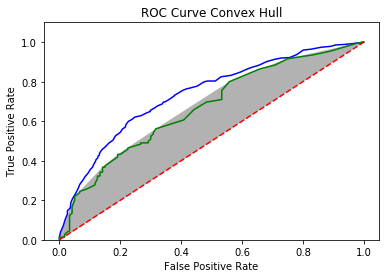
\includegraphics[width=0.5\linewidth]{imgs/convex_hull}
		\caption{The figure illustrates the intersection of the convex hulls of the conditional ROC-curves (the lower of the ROC-curves defines the border of the convex hull). The intersection is the gray area in the graph between the lower of the ROC-curves and the diagonal.}
		\label{fig:convexhull}
	\end{figure}
	\noindent
	A chosen point in the convex hull $ D_a $ represents the false and true positive rates, conditioned on a certain protected group of a randomized derived predictor based on the score function R. Due to the fact that the space of the conditional ROC-curves is two dimensional, a predictor $ \tilde Y $ can always be constructed as a mixture of two different threshold predictors. Conditioned on $ A=a $, the predictor will behave as, 
	\begin{equation}\label{odds_pred}
	\widetilde{Y}=\mathbb{I}\left\{R>T_{a}\right\},
	\end{equation}
	
	\noindent Where the variable $ T_a $ is the randomized threshold which assumes the value $ \underline{t}_{a} $ with a certain probability $ \underline{p}_a $ and the value $\bar t_{a} $ with probability $ \bar p_a $. To obtain an equalized odds predictor, a point in the intersection of the convex hull of each of the conditional ROC-curves has to be chosen and then for each group realize the true and false positive rates with a randomized predictor. For each group this results in either choosing a fixed threshold $ T_a = t_a $ or a mixture of two thresholds $ \underline t_a < t_a $. In the case of mixing two thresholds, if $ A=a $ and $ R < \underline t_a $, the predictor $ \tilde Y $ is set to 0, if $ R > \bar t_a $, the predictor is set to 1. But if $ \underline t_a < R < \bar t_a $, it is reversed and $ \tilde Y = 1 $ with probability $ \bar p_a$. Phrased in words, the sampled value, which is a random number between 0 and 1, decides whether to threshold at the upper or lower point.
	
	The equalized odds predictors is thus in the intersection of areas under the A-conditional ROC-curves, and above the main diagonal. This area is illustrated in figure \ref{fig:convexhull}. For any loss function the optimal false and true positive rate will always be on the upper left boundary. This is due to the fact that predictors close to the diagonal are no better than random. This upper left boundary is the possible equalized odds predictors. This ROC-curve, which is the upper left boundary of the intersection between the convex hulls is the point-wise minimum of the two A-conditional ROC-curves. The performance of a predictor that satisfies equalized odds is therefore determined by the minimum performance among the protected groups, which for this project are Caucasians and African-Americans. In other words, ensuring equalized odds enforces the trained model to build good predictions for all classes. For a given loss function, finding the optimal threshold can be done by optimizing ,
	\begin{equation}\label{optim_thresh}
	\min _{\forall a: \gamma \in D_{a}} \gamma_{0} \ell(1,0)+\left(1-\gamma_{1}\right) \ell(0,1)
	\end{equation}
	Assuming withouth loss of generality $ \ell (0,0) = \ell(1,1)=0 $.
	The optimization problem stated in equation \ref{optim_thresh} can be solved efficiently by numerically using ternary search. The result is two predictors for each protected attribute. For the conditional distribution, where the A-condtional ROC-curve has the lowest TPR value of the two A-conditional ROC-curves, the result will be a predictor with some threshold. Where as the other conditional population will have a predictor with a randomized threshold, see equation \ref{odds_pred}. \cite{equal_of_oppor}
	\subsubsection{Derivation of an optimal equal opportunity predictor}
	
	The construction of an equal opportunity predictor follows the same approach as \ref{optimalboi}, but has one less constraint. From the definition of equal opportunity, the predictor must only satisfy that the true positive rates are equal. This corresponds to the A-conditional ROC-curves having the same y-coordinate in the two dimensional plane. Assuming continuity of the A-conditional ROC-curves it is always possible to find points on the boundary of the conditional ROC-curves. This means that no randomization is needed, unlike when deriving an equalized odds predictor. The optimal equality of opportunity predictor corresponds to two different deterministic thresholds for each of the protected groups. The optimization problem can be solved by using exhaustive ternary search over the true positive values. \cite{equal_of_oppor} %TODO noget af hvad er siges i denne sektion er blevet nævnt, vi skal lige diskutere hvor det skal stå
	
	\subsection{Reproducibility}
	This section aims to give the reader a precise insight into how the methods of this project were implemented and how it would be possible to reproduce these results in the future. Hopefully, this will also simplify the methods. Reproducibility is an important part of writing any project or performing any research. It shows significance of the given result if it is possible for others at a later time to replicate or reproduce the results, since it validates the result of the original study and shows that it was not a fluke. All of the code is written in Python Version 3.7.4, PyTorch version 1.4.0 and Jupyter Notebook 6.0.3. Furthermore, the versions of the packages used in the project are given in the table below. All code for the project is accessible at \url{https://github.com/oskarwiese/fagprojekt/blob/master/src/Classifier_notebook.ipynb}.
	\begin{table}[H]
		\begin{center}
			\begin{tabular}{l l l l l l l l l l}
				\toprule
				& Package      & & & & & & & Version  & \\ \midrule
				& Numpy        & & & & & & & $1.16.5$ & \\
				& pandas       & & & & & & & $0.25.2$ & \\
				& matplotlib   & & & & & & & $2.2.5$  & \\
				& seaborn      & & & & & & & $0.9.0$  & \\
				& torch        & & & & & & & $1.2.0$  & \\
				& sklearn      & & & & & & & $0.0$    & \\
				& GPyOpt       & & & & & & & $1.2.5$  & \\
				& scipy        & & & & & & & $1.3.1$  & \\
				& ipywidgets   & & & & & & & $7.5.1$  & \\ \bottomrule
			\end{tabular}
		\end{center}
	\end{table}
	\noindent Since the implementation of a binary classifier and equalized odds uses random number generation, random seeds have been set in order to ensure equivalent results for every run of the notebook. The seed number was set to 42 and was used for the python seed \texttt{random.seed}, the numpy seed \texttt{np.random.seed} and the pytorch seed \texttt{torch.manual\_seed}.
	
	In order to make the results as reproducible as possible, the data as well as the way the data was obtained also plays a big role. The way the data was obtained can be seen described in detail in section \ref{dataDescription}. The data comes from the GitHub repository \url{https://github.com/propublica/compas-analysis}, from which the dataset \texttt{compas-scores-two-years.csv} was used as the only dataset for the project. \\
	
	\noindent Below, a thorough walkthrough of the most essential parts of the code will be made. To implement the bias correction methods and classifier, firstly, the dataset was loaded into a Pandas dataframe in order to easily structurize the data. Several plots of this data were then made using the Seaborn plot library. The code for this can be found in the \texttt{Data Visualization} cell. In order to pre-process the data for the implementation of a neural network, all of the features were converted into PyTorch tensors (the chosen features and order of features for this project can be seen in section \ref{Feed-forward neural}). All of the numerical variables were normalized to avoid the exploding gradient problem and to give every variable a level playing field. A FFNN was constructed using the PyTorch NN module, see the \texttt{Neural Network} cell in the notebook. The binary classifier was trained using BCE-loss with Adam as the chosen optimizer. All of the hyperparameters can be seen in section \ref{Feed-forward neural}. A permutation test was then performed to show that the acquired accuracy was adequately better than random. The classifier was used to construct predictions for conditional distributions for the protected attributes, which were saved in an array and used to construct confusion matrices at different thresholds. By using different thresholds, two  different conditional ROC-curves were constructed with Numpy and MatPlotLib. A plot of the TPR and FPR for each of the protected groups, as a function of thresholds were constructed as well, the code for which can be seen at the bottom of the \texttt{Classification} function at the top of the notebook. The next goal was to implement equalized odds and equal opportunity using these conditional ROC-curves. The code for this is located in the \texttt{BiasCorrection} function. The implementation of both equal opportunity and equalized odds is explained both by reading the code and by the pseudo code, which has been supplied in the appendix section \ref{Pseudo Equalized} and \ref{Pseudo Equal}.
	
% Forklaring af implementation af equalized odds
%	For each point on the boundary of the intersection of the convex hulls for each of the conditional distributions, the true postive and false postive rate were found. From the point on the boundary, a line was drawn between this point and the point (0,0). The slope is found using $ m=\frac{\Delta y}{\Delta x} $. Then, the intersection between the upper curve and the line was determined. The distance from (0,0) to the point on the lower curve was found and divided by the length from (0,0) to the point of the upper curve. The distance between the point on the lower curve and the intersection of the line and the upper curve is determined as well and divided by the length from (0,0) to the intersection of the line and the upper curve. This will result in two values, which are referred to as $ \bar p_a $ and $ \underline p_a $ in section \ref{optimalboi}. These are values between zero and one which will sum to one, and decides the proportion of sampling from the randomized predictor. This was done for each point on the upper left boundary of the intersection between the convex hull of the two conditional ROC-curves.

% Forklaring af implementation af equal opportunity
%As for the implementation of Equal Opportunity, it only requires that the TPR is equal for both populations. This was done by using exhaustive search, by choosing a TPR for one population, then subtracting this from the TPR-array for the other population and using \texttt{argmin} to find the one closest to zero.
	
	\section{Results}\label{results}
	%\textbf{TODO \\ dokumentér reproducerbarheden af resultaterne \\ tabeller og figurer over resultater \\ forklar resultaterne endten i diskussion eller resultater.}
	
	\subsection{Training Loss and Accuracy}
	
	\begin{figure}[H]
		\centering
		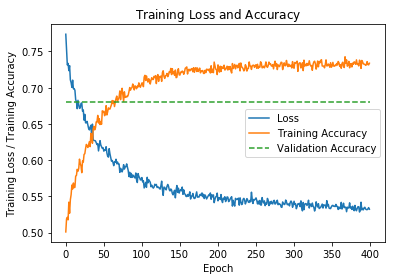
\includegraphics[width=0.5\linewidth]{imgs/loss_curve.png}
		\caption{The training loss and training accuracy after training for 400 epocs. It is clear, as expected, that the two curves are inversely proportional and that the accuracy rises with the number of epochs. After 400 epochs, the accuracy is close to having converged, but the loss still seems to get a bit lower.}
		\label{fig:losscurve}
	\end{figure}
	
	\subsection{Validation of Model Accuracy}\label{modelAccuracy}
	
	\begin{figure}[H]
		\centering
		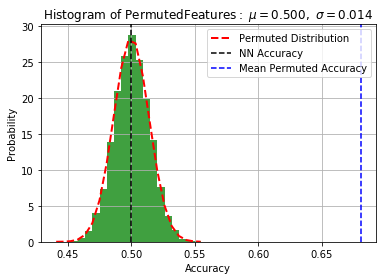
\includegraphics[width=0.5\linewidth]{imgs/perm_test.png}
		\caption{An illustration of the permutation test. The black dashed line illustrates the mean permuted accuracy, the red dashed line represents the distribution that the permuted data accuracies seem to follow and the blue dashed line is the accuracy of the model on the original non-permuted data. The standard deviation and mean represents the normal distribution which the permutations form.}
		\label{fig:permtest}
	\end{figure}\noindent
	Since the p-value cannot be 0, it is estimated by \cite{p-value}
	\[p=\frac{1}{M}=0.001.\]
	
	\subsection{Confusion Matrices}\label{confusionMatrices}
	
	\begin{figure*}[h]	
	\begin{multicols}{2}
		\begin{ceqn}
		\begin{equation*}
		\begin{bmatrix}
		193 & 103  \\
		62 & 119 
		\end{bmatrix} 
		\end{equation*} 
		\begin{equation*}
		\begin{bmatrix}
		0.412 & 0.213  \\
		0.128 & 0.246 
		\end{bmatrix} 
		\end{equation*}
		\end{ceqn}
	\end{multicols}
	{The left matrix shows the confusion matrix of the population conditioned on the Caucasian race with the threshold, $ T = 0.5 $. On the right the confusion matrix is divided by $ N_{Caucasian} $ element wise in order to show the proportions of TP, FP, TN and FN. $ N_{Caucasian} $ is the total number of Caucasians in the dataset. Below the confusion matrix, conditioned on the Afro-American population, is shown.}
	\end{figure*}
	\begin{figure*}[h]	
		\begin{multicols}{2}
			\begin{ceqn}
			\begin{equation*}
			\begin{bmatrix}
			259 & 92  \\
			165 & 231 
			\end{bmatrix} 
			\end{equation*} 
			\begin{equation*}
			\begin{bmatrix}
			0.347 & 0.123 \\
			0.221 & 0.309 
			\end{bmatrix} 
			\end{equation*}
			\end{ceqn}
		\end{multicols}
		{The threshold is set to $ T = 0.5 $. On the right the confusion matrix is divided by $ N_{Afro-American} $ element wise in order to show the proportions of TP, FP, TN and FN.}
	\end{figure*}
	
	\subsection{Conditional ROC-curves and FPR/TPR Dependency on Threshold}\label{ROC}
	
	\begin{figure}[H]
		\centering
		\begin{subfigure}{0.5\textwidth}
			\centering
			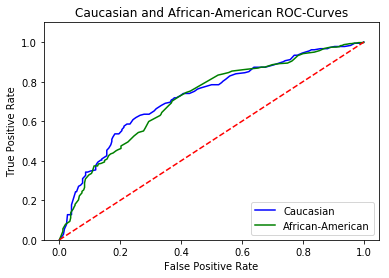
\includegraphics[width=0.9\linewidth]{imgs/ROC.png}
			%\caption{Lorem ipsum}
		\end{subfigure}%
		\begin{subfigure}{0.5\textwidth}
			\centering
			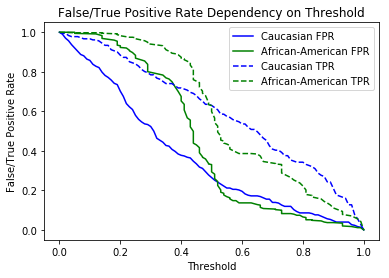
\includegraphics[width=0.9\linewidth]{imgs/fpr_tpr_plot.png}
			%\caption{An illustration of the true and false positive rates as a function of the threshold. It is clear that, although the difference in the ROC-curves seems small in plot ***, the difference in thresholds causes the true and false positive rates between the two conditional ROC-curves to be different, showing inherent bias and difference between the conditional ROC-curves.}
		\end{subfigure}
		\caption{\textbf{Left}: An illustration of the conditional ROC-Curves. Each point on the curve is realized thresholding the score function R at some value. The diagonal (the dashed red line) represents the relationship of the true positive and false positive rate for a random classifier. \textbf{Right}: An illustration of the true and false positive rates as a function of the threshold.}
		\label{fig:roc-curve}
	\end{figure}

%
	

%	\begin{figure}[H]
%		\centering
%		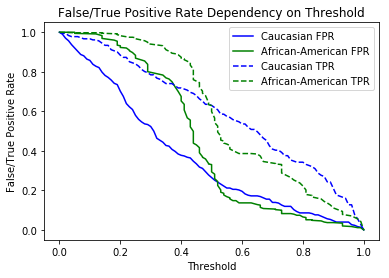
\includegraphics[width=0.5\linewidth]{imgs/fpr_tpr_plot.png}
%		\caption{An illustration of the true and false positive rates as a function of the threshold. It is clear that, although the difference in the ROC-curves seems small in plot ***, the difference in thresholds causes the true and false positive rates between the two conditional ROC-curves to be different, showing inherent bias and difference between the conditional ROC-curves.}
%		\label{fig:fprtprplot}
%	\end{figure}
		
	\subsection{Equal Opportunity}\label{equalOpportunity}
	
	\begin{figure}[H]
		\centering
		\includegraphics[width=0.5\linewidth]{"imgs/Equal Opportunity Optimal"}
		\caption{An illustration of the optimal equal opportunity threshold on the entirety of the ROC-curves. This points have equal \textit{y}-coordinates which is illustrated with the red horizontal dash line between the blue and green points. The constructed binary classifier yields an accuracy of $ 0.678 $, where the threshold used for the Caucasian is $T_{\text{Caucasian}}= 0.56 $ and the threshold for African-American is $ T_{\text{Afro-American}}=0.510 $, when equal opportunity is ensured.}
		\label{fig:equal-opportunity-optimal}
	\end{figure}
	
	\subsection{Equalized Odds}\label{equalizedOdds}
	
	\begin{figure}[H]
		\centering
		\begin{subfigure}{0.5\textwidth}
			\centering
			\includegraphics[width=0.9\linewidth]{"imgs/Equalized Odds Optimal"}
			%\caption{Lorem ipsum}
		\end{subfigure}%
		\begin{subfigure}{0.5\textwidth}
			\centering
			\includegraphics[width=0.9\linewidth]{"imgs/Equalized Odds Correctied"}
			%\caption{An illustration of the true and false positive rates as a function of the threshold. It is clear that, although the difference in the ROC-curves seems small in plot ***, the difference in thresholds causes the true and false positive rates between the two conditional ROC-curves to be different, showing inherent bias and difference between the conditional ROC-curves.}
		\end{subfigure}
		\caption{\textbf{Left}: An illustration of the line (dashed blue line) which is used to sample the best equalized odds threshold. Equalized odds entails that the TPR and FPR rates are equal. When mixing the threshold of 1 with the threshold of the blue point, a predictor which satisfies equalized odds can be found. As such, it is possible to make the false and true positive rates approximately equal. It is also clear that equalized odds and equal opportunity bias corrections methods choose almost the same threshold.  \textbf{Right}: This plot illustrates the result of the predictor which satisfies equalized odds. Hence, the blue point is moved onto the green point and thereby ensures that the TPR and FPR are approximately equal. The constructed binary classifier will yield an accuracy of $ 0.669 $, when equalized odds is ensured. The threshold for African-Americans is, $ T_{\text{African-Americans}} = 0.47 $. As for Caucasian, the predictor has a randomized threshold, $ T_{\text{Caucasian}} $. The threshold assumes the value $\underline t_{\text{Caucasian}} = 1 $  with a probability $ \underline p_{\text{Caucasian}}= 0.76 $ and the value $ \bar t_{\text{Caucasian}} = 0.50 $ with the probability $\bar p_{\text{Caucasian}} = 0.24 $.}
		\label{fig:equalizedOdds}
	\end{figure}
	
	\section{Discussion} \label{discussion}
	%\textbf{TODO: \\ etisk diskussion omkring teknologien der er arbejdet med}
	%TODO omskrive nogle af alle "Clear", så det ikke bliver for meget clearsight
	
	\subsection{Discussion of results}\label{discussionOfResults}
	This section will focus on the efficacy and reliability of the results of the project, given in section \ref{results}. From figure \ref{fig:losscurve}, it is clear that 400 epochs seems to let the binary classifier train to near completion, since the value of the binary cross-entroy training loss could still get slightly lower.%todo Kommentere på hvorfor det er vi ikke bruge mere end 400 epochs.
	Meanwhile, it is also clear that the training loss has not started rising after reaching a minimum value, so the network has not started overfitting the training data. This means that the validation accuracy will be higher after training than if the model had overfit the training data. It is also clear that the validation accuracy is lower than the training data, which is to be expected, since the model was trained to maximize success on the training and test data.
	
	From figure \ref{fig:permtest}, it is clear that the obtained accuracy is indeed significant and different from the accuracies of the permuted data, which is clear, since there are no permutations larger than the observed value. From the estimation of the \textit{p}-value in \ref{modelAccuracy}, it is obvious that the \textit{p}-value is far under the desired level of significance. Hence, the null hypothesis is rejected and the permutation test thus shows that the accuracy from the neural network on the non-permuted data is better than random and has found a meaningful interpretation of the data. This also means that the model is better than a random model (that e.g. only guesses on the largest class), so the classifier could have practical use. the accuracy of 68\% on the validation set also lines up quite well with the accuracies fround in ProPublica's analysis of the COMPAS recidivism algorithm. They found that their predictive accuracy for Caucasian and African-American defendants were 62.5\% and 62.3\% respectively, while Northpointe found accuracies of 69\% and 67\% for Caucasian and African-American defendants respectively. \cite{propublicaAnalysis}
	
	It is clear from the two normalized confusion matrices for Caucasian and African-American defendants that Caucasian defendants have almost a twice as large false positive value, while the same is true for the false negative values for African-American defendants. This signifies that the binary classifier more often labels Caucasians as not being at risk of recidivism even though they were at risk, while African-Americans are more often labeled as being at risk of recidivism when they were not truly at risk. This distinctly shows that the model is very subjective and that the original bias that seemed to be present in the data when plotting the recidivism scores for Caucasian and African-Americans, shown in section \ref{dataVisuals} and figure \ref{fig:predictedrecidrace}, has been learned by the model as well. This shows that care needs to be taken to avoid biased datasets or to implement the necessary steps like bias correction methods to avoid bias in the model before, during or after training. Meanwhile though, care needs to be taken when dealing with bias removal, as it is also necessary to prove that the bias is unjustified in the data. This was attempted proven in this project using figure \ref{fig:truerecid}, which shows that the discrepancy in amounts of Caucasian and African-American defendants is not as large as would be expected from figure \ref{fig:predictedrecidrace}. As such, it makes sense to attempt to correct this bias.
	
	The conditional ROC-curves from section \ref{ROC} figure \ref{fig:roc-curve} may at first glance seem very similar, but when the dependency of the specific threshold is taken into consideration, it is clear that there are major differences. The difference in thresholds causes the true and false positive rates between the two conditional ROC-curves to be different, showing an inherent bias and of course a difference between the conditional ROC-curves. This confirms the suspected bias seen from figure \ref{fig:predictedrecidrace} and \ref{fig:proirs} in the data section. Since the two ROC-curves are different, using just one common threshold for both races would result in a biased model, exactly what happened in Northpointe Inc.'s algorithm. For this reason, equal opportunity or equalized odds with a threshold for each protected attribute (Caucasians and African-Americans in this case) needs to be used, sometimes even when the curves look deceivingly similar.
	
	In section \ref{equalOpportunity} figure \ref{fig:equal-opportunity-optimal} equal opportunity has been implemented to correct the present bias in the model. It is clear that the middle of the ROC-curves seems to yield the best accuracy, which is reasonable, since a classifier with higher true positive rate and lower false positive rate will have a higher accuracy. This also implies that the trivial endpoints, at which the false and true positive rates are already equal, will not bring much value when optimizing for an unbiased model with high accuracy, as the accuracy in these points will be very close to random. As for the implementation of equalized odds in figure \ref{fig:equalizedOdds} from section \ref{equalizedOdds}, it is clear that the same is true, since almost the same points and thresholds have been chosen to maximize accuracy while keeping the condition of equalized odds. In the case of accuracy reduction, it seems that both methods only carry with them a small decrease in accuracy. The accuracy of the original biased binary classifier is 68.3\%. This accuracy is reduced to 67.8\% using equal opportunity and to 66.9\% using equalized odds. From this, it is obvious that equalized odds takes a bigger hit on accuracy, though the differences in accuracy is still 0.5\% for equal opportunity and 1.4\% for equalized odds, so the overall loss in accuracy definitely seems to be worth it to get a properly working model that does not discriminate on any of the protected attributes.
	
	\subsection{Ethical dilemma of bias}
	
	\subsubsection{Where does bias come from?}\label{rootofbias}
	Bias is defined in the dictionary as \textit{\enquote{inclination or prejudice for or against one person or group, especially in a way considered to be unfair.}} In general bias can be natural or innate,  but can also be learned. Bias can be developed by humans for or against people, certain individuals, objects, beliefs or even cultures. Several type of cognitive biases exist. A cognitive bias is a systematic error in thinking that occurs when people are processing and interpreting information in the world around them and affects the decisions and judgments that they make. \cite{verywellmind} A few example of these are: Confirmation bias, the Halo and Horn effect and Misinformation effect. Confirmation bias is the favoring of information that confirms one's own belief and discounting information that opposes or challenges one's belief. The Halo and horn effect is the effect of how an overall impression of someone influences how one feel and think about the someone. This effect can both be positive and negative, and hence shows the importance of first impression. The misinformation effect is the tendency of information that happens post an event to interfere with the memory of the original event. Besides, the three mentioned biases a lot of others exist, and all of these biases have consequences of how we as humans make decisions and judge other people. Considering a court room, where an evaluation of whether a defendant should be let out on parole or not, is taking place. Imagine how the Misinformation effect influences the defendants memory processing or how confirmation bias or the halo effect influences the jurisdiction of the judge. Studies also show, that being hungry affects judgement  and how one make decisions. \cite{eat}. \newline \indent
	The consequences of cognitive biases can lead to distorted thinking. Often conspiracy theories as well as extremists political beliefs stems from cognitive biases which can lead to very irrational beliefs. \cite{cog_bias} Humans are thus in general very biased and are affected by bias every day of their life. The question is then, if bias is necessarily a bad thing. In psychology it is a well accepted theory, that many of the cognitive biases serve humans to optimize our way of living. Among others by allowing decisions within milliseconds which can be vital in dangerous situations. \cite{reisberg} However, bias can also be discriminating, as bias and prejudice are closely related. Prejudice is prejudgment, which is forming an opinion of someone or something beforehand. Prejudice and biases can lead to racism and sexism, which is why detecting bias is such an important topic. In conclusion, data that has been generated by humans, i.e. the COMPAS dataset, will be biased and needs to be properly handled in order to ensure fair ML models.
	
	\subsubsection{Who does bias affect and why do we care about fairness?}
	As mentioned in section \ref{rootofbias} all humans are affected by bias. However, when considering the the question of who it affects, it refers to the protected groups. This is minority groups in society and undiscovered biases can have major impacts as machine learning plays a greater role in the every day life of humans. For instance its important to ensure that the opportunity of getting a loan is equal for all genders and races. Using historical data from the past to train machine learning models to determine the probability of a person getting a loan can lead to sexist and racist models that reject women or African-Americans when they apply for a loan in the bank. This problem stems from racist and sexist behavior of human beings in the past and therefore this study calls for the importance of acknowledging biased human behavior. Machine learning models are often viewed as objective whereas this often can be misleading. The results found in this study confirms the opposite, which proves that a model inherent bias from the data used to train the model. Machine learning models are implemented in several areas of society including self driving cars, healthcare industry, public safety, retail sector and more.Thus, ensuring fairness in machine learning models is important to make the decision of all models comply with the declaration of human rights (The declaration of human rights can be found at \url{https://www.un.org/en/universal-declaration-human-rights/}).
	
	\subsection{Examination of fairness definitions}
	The fairness definitions that have been implemented in this project can be seen in section \ref{bias_def}. These are definitions which are proposed by Mortiz Hardt et al. and this section will thoroughly discuss these. Equality of opportunity states, that the true positive rate for all groups has to be equal. Consider a hiring algorithm designed to pick the best applicants for a certain job (a real life example of this is Amazon which tried to create a job hiring algorithm, see an article by \href{https://www.reuters.com/article/us-amazon-com-jobs-automation-insight/amazon-scraps-secret-ai-recruiting-tool-that-showed-bias-against-women-idUSKCN1MK08G}{Reuters} for more information if desired. However, this is not relevant for this section). If there are two groups, A \& B, of applicants which both consists of 100 people each. Furthermore, if $ 58 $ people in group A are qualified for the job whereas $ 2 $ people in group B are qualified for the job, and both groups apply for the job. Then, equalized odds states if $ 30 $ people are to be hired then $ 29 $ people from group A should be hired whereas $ 1 $ from group B should be hired, in order for the algorithm to ensure equal opportunity. \cite{towardsdata} If this was a high end job at Google, then group A would have a higher living standard than B. Group A would afford better education for their children, more expensive houses or apartments and so on. This leads to the algorithm, which according to Hardt ensures fairness, to create a larger gap between to possible groups in society. One could then ask if creating a larger gap between groups, resulting in a society with a superior elite, is in any means a way to create fair machine learning models. \newline
	\\
	\noindent 
	The pressing issue of creating a gap between groups is applicable for equalized odds since this notion of fairness require the true positive rates to be equal as well. Furthermore, the stronger notion, equalized odds, requires the false positive rates of two groups to be equal. This constraint enforces a good classifier to be good at predicting all classes in order to achieve a pinnacle accuracy. This could potentially be an advantage that will ensure models used in society are fair. This will be elaborated in section \ref{tradeoff} .  
	
		\subsection{Trade-off between accuracy and fairness}\label{tradeoff}
	Normally, when correcting for bias in a binary classifier, the accuracy will take a hit to some extent. This happens because the optimal predictor from both of the groups will probably not be chosen when the true or true and false positive rates have to be equal. This also has to be true because two classifiers are forced to have the same false and true positive rates, which means that the accuracy will be the same over all protected groups, so the lower of the accuracies will be fixed as the accuracy for both of the protected attributes. This is not true in the same sense in equal opportunity, as this methods chooses the values with the same true positive rate only. As such, it is possible for the upper of the two curves to utilize the better accuracy, which still ensuring some bias correction. As such, only a slight loss of accuracy will be observed. \cite{equal_of_oppor} This can be seen in our project from section \ref{equalOpportunity} and section \ref{equalizedOdds} from figures \ref{fig:equal-opportunity-optimal} and \ref{fig:equalizedOdds}. The accuracy difference of these methods has also been described in section \ref{discussionOfResults}. Here, it is clear that the difference in accuracy between the biased model and equalized odds-corrected model is larger than between the biased model and equal opportunity-corrected model, as is to be expected. In the case of this project though, the differences in accuracies of 0.5\% and 1.4\% is still more than low enough for the bias correction to be worth it, as the non-discrimination also makes the model more accurate for practical use in return.
	%\subsection{Avoidance of responsibility}
	
	To better quantify the differences in accuracy between a binary classifier and a random classifier as well as finding the true discrimination of a model, Indrė Žliobaitė proposes that the accuracy difference can be found using Cohen's Kappa, which normalizes the accuracy of the model based on the value of the random classifier accuracy. He also proposes normalizing the discrimination (which, in this case, is defined as the difference between true positives in the protected groups) by the highest discrimination value over all thresholds, as this ensures that the discrimination reaches a maximum if the binary classifier first accepts everyone from the favored protected attribute and only then starts accepting individuals from the non-favored attribute. This finding could make sense to look into for further work into this project, as the true model difference from a baseline or random model would have significance, when attempting to communicate the effectiveness of the model. \cite{bias-accuracy}
	
	\subsection{Why do we care about fairness?}
	The thoughts of discrimination and notions of fairness within the field of machine learning came vastly later than the methods itself. An important question to shed light on is why the concept of fairness is important and which impact the definitions we make now have on the future of the world. In the modern society we live in today most AI-models implemented commercially are supervised learning models which all learn from data. However, in future settings models will have to make a wider extent of decisions such as controlling traffic lights, driving cars, engaging with lonely individuals and more. At some point in time the human race will develop superintelligence, which is defined as an intelligence which is significantly higher than that of humans. \cite{superint} When the human race reaches this pinnacle of inventions we need to have mastered and defined the utmost notions of fairness. A superintelligence will make vital decisions such as whether to wage war, what a country should invest in and much more. Therefore, notions such as equalized odds will not work as this ultimately could create a gap in society and result in forming an elite that controls the outcome of society as a whole. This study calls for more attention to developing a notion that ensures fairness meanwhile we live in a world where consequences are merely unfair treatment. The discrimination that are present in the world today is due to models such as the one commercialized by Northpointe Inc., and this pressing issue grows as the knowledge and studies of fairness in machine learning grows. One of the many reasons why discriminating models are allowed to exist is due to the lack of regulation on machine learning models. Take for instance Rigshospitalet (The National, State or Kingdom Hospital of Denmark) into consideration, where there currently, are no regulation on presently used  machine learning models. These are models that primarily are trained on young Caucasian males, and at time of classification of an elderly Afro-American women, there is no law or anything that ensures that no discrimination is happening or that the classification is fair under any notion of fairness. The machine learning models used in the medical industry are only pin pointers that assist the educated doctor that has the final say. However, due to known cognitive biases such as anchoring which can affect the outcome a doctor the study also calls for proper laws and regulation on the topic of commercialized machine learning models.
	\\\\
	In conclusion, we care about fairness because discrimination is happening right now which is a pressing issue in society. With no laws or regulations a rise in discriminatory classifiers and machine learning models happens for every day that passes by. A lot of people can be unaware that they are being treated unfair which is why shedding light on this topic will have a meaningful impact on the common good of the world. Furthermore, proper notions of fairness, regulations and laws has to be made in order for the possibility of developing artificial intelligence which acts as a part of society. A solution can be an UN-body which will be able to pass resolutions with proper regulations and fairness notions. The UN-body can furthermore act as a council which ensures that all models fulfill the deceleration of human rights and future resolutions. 
	
	
	\subsection{The value alignment problem}
	
	
	\subsection{Safe AI}
	
	

	
	\section{Conclusion} \label{conclusion}
	%\textbf{TODO: \\ Opsummér resultater og anbefalinger fra projektet \\ Må ikke indeholde noget nyt \\ Skal svare på spørgsmålene fra problemformuleringen \\ Konklusion, abstract og indledning skal give samlet billede af projektet}
	Generally, after having implemented the bias correction methods equal opportunity and equalized odds, a few things have come to light. Firstly, it is clear that the data could be crooked when looking at section \ref{dataVisuals} figure \ref{fig:predictedrecidrace}. It is seen that Caucasians are 1.5 times as often classified as belonging to the class of low recidivism risk, while African-Americans are more than twice as often labeled as having high risk of recidivism than Caucasians. As such, the data seems to have a bias towards rating African-Americans as having higher risk of recidivism. The same cannot be said for sex, though, as it can be seen from figure \ref{fig:predictedrecidsex} that males and females are treated approximately equal. The conclusion of this section is thus that only a bias between Caucasians and African-Americans exists in the data. By bias in the data, it is simply meant that some protected group is treated unfairly compared to another. The only true way to analyse whether this is the case, is to look at histograms for both of the protected groups. This is not a bulletproof methods but supplies a point of suspected bias, which can be analyzed using the methods covered in section \ref{methods}.
	
	As can be understood from section \ref{confusionMatrices}, the bias that is suspected to exist in the data rears it head in the binary classifier too, further signifying the actual existence of this bias. The fact that the classifier is biased is shown by comparing the false negative and false positive values of these confusion matrices, as this signifies that the model is attempting to place more Caucasians in the positve class and more African-Americans in the negative class, which is a biased viewpoint, since neither the Caucasians or the African-Americans in the false positive and false negative actually belong there. Meanwhile, the true positive and true negative values do not express bias, as this is the actually recidivism pattern seen in the data. Looking at the conditional ROC-curves and false/true positive rate dependencies on threshold from figure \ref{fig:roc-curve}, the model is also shown to be biased, since the same threshold for the two protected groups yield widely differing true positive and false positive rates. Thus, another way to find bias in the algorithm is to show the ROC-curves of each protected group.
	
	As can be seen in figure \ref{fig:equal-opportunity-optimal} and \ref{fig:equalizedOdds}, equal opportunity and equalized odds have been implemented to great success. The accuracy is still high and African-Americans are now no longer getting discriminated upon by the binary classifier, since the bias correction methods have ensured equal true or true and false positive rates. As such, African-Americans are now equally as often as Caucasians given the label of low or high risk of recidivism. This change was made with little penalty made to the accuracy, as equal opportunity resulted in a drop in accuracy of 0.5\% and equalized odds resulted in a 1.5\% drop in accuracy. As such, for this project, it is definitly worth it to make the model less biased for such a small decrease in accuracy. 
	
	\begin{enumerate}	
		\item Which applications can bias-correction algorithms as well as AI-models have in society? And how can society gain trust in these models? 
	\end{enumerate}
	
	\section{Appendix} \label{appendix}
	
	\begin{figure}[H]
		\centering
		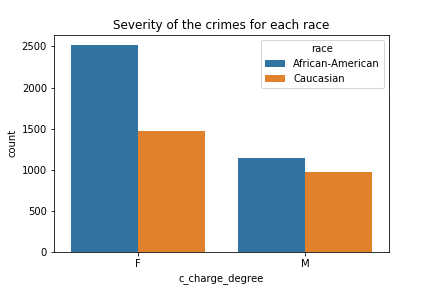
\includegraphics[width=0.5\linewidth]{imgs/c_charge_degree}
		\caption{}
		\label{fig:cchargedegree}
	\end{figure}
	
	\begin{figure}[H]
		\centering
		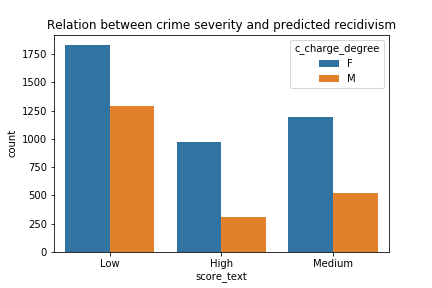
\includegraphics[width=0.5\linewidth]{imgs/charge_degree_score}
		\caption{}
		\label{fig:chargedegreescore}
	\end{figure}
	\subsection{Pseudo Code}
	\subsubsection{Equalized Odds}\label{Pseudo Equalized}
	The implementation of equalized odds below assumes that the ROC-curve belonging to the \texttt{fprs1} and \texttt{tprs1} values is always placed above the other ROC-curve in order to save space, as the implementation is similar for having the curves overlap. The \texttt{accuracy\_score} function used in this implementation is the function from \texttt{sklearn.metrics}. The documentation can be seen here: \url{https://scikit-learn.org/stable/modules/generated/sklearn.metrics.accuracy_score.html}.
	\begin{lstlisting}[escapechar=@,escapebegin=\itshape]
	def EqualizedOdds(fprs1, fprs2, tprs1, tprs2, true1, true2, probs1, probs2, ...
	                  thresholds1, thresholds2, points):
	                  
	  # @Calculates the equalized odds predictors for two ROC-curves.@
	  # @Parameters:@
	  #    @\textbf{fprs1(list), tprs1(list), fprs2(list), tprs2(list):} False/true positive values for upper@
	  #    @and lower curve respectively.@
	  #    @\textbf{true1(list), true2(list):} The labels for the actual recidivism values.@
	  #    @\textbf{probs1(list), probs2(list):} the probabilities for 0 or 1 recidivism given by the classifier.@
	  #    @\textbf{thresholds1(list), thresholds2(list):} The thresholds used to construct the ROC-curves.@
	  #    @\textbf{points(int):} The number of points used to construct the ROC-curves.@
	  # @Returns:@
	  #    @\textbf{bestAcc(float):} Value of the best accuracy.@
	  #    @\textbf{percentage(float):} The percentage of times the non-1 threshold is sampled.@
	  #    @\textbf{bestThreshold1(float), bestThreshold2(float):} The thresholds used for@
	  #    @the two curves.@
	  
	  accs = empty list of size points
	  thresholdOrder = empty list of size points
	  for pointIndex from 0 to points:
	    # @Defining a line going through (0,0) and the desired point on the lower curve@
	    slope = tprs2[pointIndex] / fprs2[pointIndex]
	    def line(x):
	      return slope * x
	    linediff = abs(tprs1 - line(fprs1))
	    # @Find the intersection of the line and upper curve, considering only points to the right@
	    # @of the lower intersection@
	    intersectionIndex = argmin(linediff[line(fprs1) > tprs2[pointIndex]])
  	    x1 = fprs1[intersectionIndex]
	    x2 = fprs2[pointIndex]
	    y1 = tprs1[intersectionIndex]
	    y2 = tprs2[pointIndex]
		
	    # @Define thresholds and find line lengths to sample from the thresholds@
	    thres1 = 1.0
	    thres2 = thresholds1[intersectionIndex]
	    thresholdOrder[pointIndex] = thres2
	    fullLength = sqrt(y1^2 + x1^2)
	    firstLength = sqrt(y2^2 + x2^2)
	    secondLength = fullLength - firstLength
		
	    sampleThreshold = firstLength / fullLength
	    yPred1Low = if probs1[i] > thres1[i] then 1 otherwise 0 for every value in probs1
	    yPred1High = if probs1[i] > thres2[i] then 1 otherwise 0 for every value in probs1
	    yPred1 = empty list of size probs1
	    for i from 0 to length of yPred1:
	      sampleValue = uniform distribution sample between 0 and 1
	      if sampleValue > sampleThreshold:
	        yPred1[i] = yPred1Low[i]
	      else:
	        yPred1[i] = yPred1High[i]
	    yPred2 = if probs2[i] > thresholds2[i] then 1 otherwise 0 for every value in probs2
	    acc = accuracy_score(true1, yPred1) + accuracy_score(true2, yPred2)) / 2)
	    accs[i] = acc
	  bestIndex = argmax(accs)
	  bestAcc = accs[bestIndex]
	  percentage = 1-sampleThreshold
	  bestThreshold1 = thresholds1[bestIndex]
	  bestThreshold2 = thresholdOrder[bestIndex]
	  return bestAcc, percentage, bestThreshold1, bestThreshold2
	\end{lstlisting}
	
	\subsubsection{Equal Opportunity}\label{Pseudo Equal}
	The \texttt{accuracy\_score} function used in this implementation is the function from \texttt{sklearn.metrics}. The documentation can be seen here: \url{https://scikit-learn.org/stable/modules/generated/sklearn.metrics.accuracy_score.html}.
	\begin{lstlisting}[escapechar=@,escapebegin=\itshape]
	def EqualOpportunity(fprs1, tprs1, fprs2, tprs2, true1, true2, probs1, probs2, ...
	                     thresholds1, thresholds2, points):
	                     
	  # @Calculates the equal opportunity predictors for two ROC-curves.@
  	  # @Parameters:@
	  #    @\textbf{fprs1(list), tprs1(list), fprs2(list), tprs2(list):} False/true positive values for upper@
	  #    @and lower curve respectively.@
	  #    @\textbf{true1(list), true2(list):} The labels for the actual recidivism values.@
	  #    @\textbf{probs1(list), probs2(list):} the probabilities for 0 or 1 recidivism given by the classifier.@
	  #    @\textbf{thresholds1(list), thresholds2(list):} The thresholds used to construct the ROC-curves.@
	  #    @\textbf{points(int):} The number of points used to construct the ROC-curves.@
	  # @Returns:@
	  #    @\textbf{bestAcc(float):} Value of the best accuracy.@
	  #    @\textbf{bestThres1(float):} Value of the threshold for the upper curve with highest accuracy.@
	  #    @\textbf{bestThres2(float):} Value of the threshold for the lower curve with highest accuracy.@
	  
	  accs = empty list of size points
	  thresholdOrder = empty list of size points
	  for pointIndex from 0 to points:
	    x2 = fprs2[pointIndex]
	    y2 = tprs2[pointIndex]
	    ydiff = abs(y2 - tprs1)
	    intersectionIndex = argmin(ydiff)
	    x1 = fprs1[intersection_idx]
	    y1 = tprs1[intersectionIndex]
	  
	    thres1 = thresholds1[intersectionIndex]
	    thresholdOrder[pointIndex] = thres1
	    thres2 = thresholds2[pointIndex]
	    yPred1 = if probs1[i] > thres1[i] then 1 otherwise 0 for every value in probs1
	    yPred2 = if probs2[i] > thres2[i] then 1 otherwise 0 for every value in probs2
	    acc = accuracy_score(true1, yPred1) + accuracy_score(true2, yPred2)) / 2
	    accs[pointIndex] = acc
	  bestIndex = argmax(accs)
	  bestAcc = accs[bestIndex]
	  bestThres1 = thresholdOrder[bestIndex]
	  bestThres2 = thresholds2[bestIndex]
	  return bestAcc, bestThres1, bestThres2
	  
	\end{lstlisting}
	
	\begin{thebibliography}{9} \label{bibliography}
		
		\bibitem{bo_lib} Machine Learning Group, University of Sheffield: "GPyOpt’s documentation", at \url{https://gpyopt.readthedocs.io}
		
		\bibitem{equal_of_oppor} M. Hardt, E. Price, and N. Srebro. Equality of Opportunity in Supervised Learning. In NIPS, 2016.
		
		\bibitem{Zafar} M. B. Zafar, I. Valera, M. G. Rodriguez, and K. P. Gummadi. Fairness constraints: A mechanism for fair classification.
		In ICML Workshop on Fairness, Accountability, and Transparency in Machine Learning, 2015.
		
		\bibitem{floridaLaw} The State of Florida, "The 2019 Florida Statutes", 1995,  \url{http://www.leg.state.fl.us/statutes/index.cfm?App_mode=Display_Statute&URL=0100-0199/0119/0119.html}, visited 12-03-2020
		
		\bibitem{propublicaAnalysis} ProPublica, "How We Analyzed the COMPAS Recidivism Algorithm", 2016, \url{https://www.propublica.org/article/how-we-analyzed-the-compas-recidivism-algorithm}, visited 12-03-2020
		
		\bibitem{aktiv_gp} F. Bergamin. 02463 “Active Machine Learning and Agency” Lecture 1: Gaussian Processes, 2020.
		
		\bibitem{aktiv_bo} F. Bergamin. 02463 “Active Machine Learning and Agency” Lecture 2: Bayesian Optimization, 2020.
		
		\bibitem{dl} Goodfellow-et-al-2016. Deep Learning, MIT Press in 2016. 
		
		\bibitem{b_woodworth} B. Woodworth et al. Learning Non-Discriminatory Predictors, Toyota Technological Institute at Chicago, Chicago, IL 60637, USA; Proceedings of the 2017 Conference on Learning Theory.
		
		\bibitem{g_goh} G. Goh et al. Satisfying Real-world Goals with Dataset Constraints. In NIPS, 2016.
		
		\bibitem{p-value} Phipson, Belinda and K. Smyth, Gordon "Permutation P-values Should Never Be Zero: Calculating Exact P-values When Permutations Are Randomly Drawn", Walter and Eliza Hall Institute of Medical Research, 31. October 2010.
		
		\bibitem{verywellmind} Verywell Mind, "What Is Cognitive Bias?", 05 May 2020,
		\url{https://www.verywellmind.com/what-is-a-cognitive-bias-2794963#:~:text=A%20cognitive%20bias%20is%20a,and%20judgments%20that%20they%20make.}, visited 08-06-2020
		
		\bibitem{eat} P. Hunter Your decisions are what you eat. Metabolic state can have a serious impact on risk-taking and decision-making in humans and animals. EMBO Rep. 2013
		
		\bibitem{cog_bias} Žeželj, I., \& Lazarević, L. B.  Irrational Beliefs. Europe’s Journal of Psychology, 15(1), 1-7 2019.
		
		\bibitem{reisberg} D. Reisberg Cognition chapter 12 - Judgement and Reasioning, sixth edition (2015)
		
		\bibitem{towardsdata} Ziyuan Zhong, "A Tutorial on Fairness in Machine Learning" 2018, \url{https://towardsdatascience.com/a-tutorial-on-fairness-in-machine-learning-3ff8ba1040cb}, visited at 08-06-2020
		
		\bibitem{bias-accuracy} Indre Zliobaite. On the relation between accuracy and fairness in binary classification. CoRR, abs/1505.05723, 2015.
		
		\bibitem{superint} Nick Bostrom, "Superintelligence" Oxford University Press, 29-03-2016
		
	\end{thebibliography}
	
	
	\newpage
	\bibliographystyle{IEEEbib}
	\bibliography{refs}
\end{document}
